%
\documentclass[referee]{aa} % for a referee version
%\documentclass[onecolumn]{aa} % for a paper on 1 column  
%\documentclass[longauth]{aa} % for the long lists of affiliations 
%\documentclass[letter]{aa} % for the letters 
%\documentclass[bibyear]{aa} % if the references are not structured 
%                              according to the author-year natbib style


%\documentclass{aa}  
\usepackage{hyperref}
\usepackage{graphicx}
%%%%%%%%%%%%%%%%%%%%%%%%%%%%%%%%%%%%%%%%
\usepackage{txfonts}
%\usepackage{multirow}
%%%%%%%%%%%%%%%%%%%%%%%%%%%%%%%%%%%%%%%%
\usepackage{subcaption}
\usepackage{flushend}
  % results heading (mandatory)
\begin{document} 


   \title{Data processing pipelines and the data platform for the X-ray spectrometer/imager STIX onboard Solar Orbiter}

   \subtitle{}

   \author{Hualin Xiao
          \inst{1}
          \and 
          Shane Maloney 
          \inst{2}
          \and S\"am Krucker\inst{1}
          \and Paolo Massa \inst{6}
          \and Lastufka Erica \inst{1}
          \and Ewan Dickson \inst{4}
          \and Andrea Francesco Battaglia\inst{3}
          \and Frederic Schuller \inst{7}
          \and Ryan Daniel \inst{1}
          \and László Etesi \inst{1}
          \and Nicky Hochmuth \inst{1}
          \and Collier Hannah \inst{1}
          \and Olivier Limousin \inst{5}
          \and Gordon Hurford\inst{1} 
     %     \and Astrid M. Veronig\inst{4} 
          \and Alexander Warmuth \inst{7}
          \and other STIX data center contributors
         }

   \institute{University of Applied Sciences and Arts Northwestern Switzerland (FHNW), 5200 Windisch, Switzerland \\
              \email{hualin.xiao@fhnw.ch}
         \and
          Astrophysics Research Group, School of Physics, Trinity College Dublin, Dublin 2, Ireland
          \and
             ETH Z\"urich, R\"amistrasse 101, 8092 Z\"urich, Switzerland
         \and University of Graz, Universitätspl. 3, 8010 Graz, Austria
         \and IRFU, CEA, Université Paris-Saclay, and Université Paris Diderot, AIM, Sorbonne Paris Cité, CEA, CNRS, 91191 Gif-sur-Yvette,
         France
         \and Dipartimento di Matematica, Università degli Studi di Genova, Via Dodecaneso 35, 16146 Genova, Italy
         \and Leibniz-Institut für Astrophysik Potsdam (AIP), An der Sternwarte 16, D-14482 Potsdam, Germany
             }

   \date{\today}

% \abstract{}{}{}{}{} 
% 5 {} token are mandatory
 
  \abstract
  % context heading (optional)
   { The Spectrometer/Telescope for Imaging X-rays (STIX) instrument is one 
   of the ten instruments onboard the Solar Orbiter to measure spectra and take images of solar flare X-rays in the energy range of 4 to 150 keV over a wide range of sizes.} %leave it empty if necessary  
  % {context.}
  % aims heading (mandatory)
   {During nominal operation, STIX continuously generates data. Constant data flow requires fully automated data processing pipelines to process,
     analyze the data and a data platform to manage, 
   visualize and distribute STIX generated by the pipelines.   
   }
   {
   A data center has been established at FHNW. 
   It consists of automated pipelines and a data platform.
   The pipelines process telemetry data, perform standard scientific analysis 
    , and generate data products at different levels.  
   The software running on the platform 
   consists of databases and web-based applications. The platform provides application interfaces for STIX data users. }
   {
 The platform provides  all STIX data products of different levels and also provides users 
 with various web-based tools for searching for, downloading and  browsing STIX data products, 
 and performing common analysis tasks with STIX data. 
  The data center is designed to operate in a fully automated mode with minimal human intervention. The concept has proven successful 
 and has been running continuously for more than two years. The platform not only facilitates instrument operations but also provides great support to STIX data users.}
 {}
\keywords{Solar flares -- Data platform --
                STIX data products --
                -- X-ray imaging, 
                Data processing pipeline
               }
  \titlerunning{STIX data center}
  \authorrunning{Hualin Xiao and STIX team}
   \maketitle

%-------------------------------------------------------------------

\section{Introduction}
Solar Orbiter is a Sun-observing mission of the European Space Agency that 
addresses the interaction between the Sun and the heliosphere.
It was launched on Feb. 10, 2020, for a nominal mission duration of seven years and a planned 
extension of three years. It carries ten sets of instruments for comprehensive
remote sensing and in-situ measurements. 
Solar Orbiter will perform detailed measurements of the Sun as close as 0.28 AU and for the first time look at its uncharted polar regions (\cite{SolarOrbiter2020}).  
The Spectrometer Telescope for Imaging X-rays (STIX) is one of the ten instruments onboard the Solar Orbiter.  
It measures X-rays from 4 to 150 keV and takes X-ray images with a few arcsec angular resolutions by using an indirect imaging technique based on the Moiré effect.  The STIX instrument consists of 32 collimators with grids and 32 pixelated cadmium telluride detectors.  The main science objective of STIX is to study the extremely hot solar plasma and the high-energy electrons accelerated during solar flares. STIX provides intensity,  spectrum, timing, and location of accelerated electron information of solar flares. For more information on STIX instrumentation and its scientific capabilities, we refer to the instrumentation paper (\cite{StixInstrument}).


During normal operations, STIX continuously acquires data. To reduce the amount of data that needs to be transmitted, STIX compresses and formats the data into different types of telemetry packets on board. 
The total number of telemetry packets can reach hundreds. To assist with the complexity of STIX data analysis and make the data more accessible to the solar physics community, automated data processing pipelines and a data platform have been developed at FHNW. The pipelines convert raw telemetry data into quick-looks and data products at different levels that can be used for scientific analysis. The platform stores all STIX data products and provides web-based tools for users to explore and analyze STIX data.

 The purpose of this paper is to describe the processing pipelines,
 the core algorithms of standard analysis, the STIX data products, and the tools provided by the 
 STIX data platform for STIX data users.

\section{STIX raw telemetry data}
\label{sec:raw-data}
When STIX is in the normal observation mode, it continuously records signals from the X-ray detectors, aspect system, and housekeeping sensors.  
After signals are processed by the onboard FPGA and CPU, three types of data are generated: housekeeping (HK) data,  quick-look (QL)  data, and scientific data.
Housekeeping data and quick-look data low-latency telemetry data are sent to storage on the spacecraft, while high-time resolution pixel data are written to the STIX onboard archive memory for a later generation of science data after receiving data request telecommands from the ground. STIX generates hundreds of different types of telemetry data, but from the perspective of data users, there are tens of the most important data types that can be grouped into three categories: housekeeping data, quick-look data, and science data.
\subsection{Housekeeping data}
Housekeeping (HK) data are generated as long as STIX is on.
A housekeeping packet contains information on the instrument,  such as temperature,
voltage, current, the status of switches, CPU usage, onboard flash memory usage, 
detector median and maximum trigger rates, and readouts from the four photodiodes.
During nominal operation, STIX generates a housekeeping every 64 seconds, 
resulting in daily raw telemetry of 143 KiB.
Housekeeping data not only provide instrument status information but also 
pointing information, which can be derived from the aspect system readouts. 
Housekeeping data are down-linked to the ground with the highest priority and are available on the platform
within 24 hours. 

\subsection{Quick-look data}
STIX generates four different types of quick-look data in NOMINAL mode (regular science mode):
\begin{itemize}
\item Light curve data contain time series 
of detector-summed counts (Counts recorded for the two 
special detectors  the background monitor and the coarse flare detector are excluded) 
in five different energy bands, rate control regions, and detector-summed triggers 
integrated over 4 seconds. Note that counts are not corrected for dead time,  transmission, impacts of the presence of the attenuator, 
or rate control regimes.

\item Background data. 
The BKG subcollimator consists of an open front grid window
and a rear grid window that is fully opaque except for six small
apertures. It is used to measure background and incident flux when other detectors are saturated.  
Background data contain counts and trigger sum over BKG pixels and integrated over 8s in the five energy
bands the same as those of QL light curves. 
\item Variance data are the onboard computed variance of 40 successive detector-summed count rates
based on 0.1-second integration.
\item Quick-look spectra. Quick-look spectra 
 are energy snapshots of energy spectra (32 science energy bins) for
each of the 32 detectors with 32 s exposure time.
STIX takes a snapshot of energy spectra every 1024
seconds during nominal operation.
\item Calibration data. 
Calibration data contain high-resolution raw energy spectra of each pixel accumulated for 
events emitted by 128 weak $^{133}$Ba radioactive sources. 
They are used to determine the energy conversion factors of each pixel by using photopeaks in the calibration spectra.  
During nominal operations, a calibration run typically lasts about 24 hours, and a new calibration run is started immediately. 

\end{itemize}


\subsection{Bulk science data}

Bulk science data are different combinations of summing and compression of the raw pixel data stored in STIX 
onboard archive memory, which is only generated after receiving data request commands from the ground. 
STIX generates six different types of bulk science data: 
\begin{itemize}
 \item Raw pixel data: Raw pixel data are the least processed data and contain
  uncompressed counts for the selected energies, pixels, and detectors; 
\item Pixel data are essentially the same as raw pixel data, 
but the counts are compressed onboard before being sent to the spacecraft;
\item Compressed pixel data are further compressed counts from the pixel data,
 in which are summed down to 4 before compression.
\item Visibilities further reduces the data by combining the four summed pixel counts into complex visibility, 
which is also compressed.
\item Spectrograms are detector summed spectrograms; 
\item High-time resolution readouts of photodiodes in the aspect system;
\end{itemize}
Bulk science data are sent to the ground in the format of raw binary packets and  are
considered level-0 at the STIX data center.  


%The coverage, data rate, and latency of 
%different types of STIX raw telemetry data are
%summarized in Table \ref{tb:raw_types}.
%https://issues.cosmos.esa.int/solarorbiterwiki/display/SOSP/SOC+Archive+Plan?preview=%2F11734040%2F21759347%2FSOL-SGS-PL-0009-SOARPL-2.0.pdf

\section{Data reception}

During nominal science operations, low-latency data (housekeeping data, quick-look data and calibration data)
are down-linked to 
the very next ground station pass regardless of orbital geometry, 
whereas science data are only down-linked when the bandwidth permits.
Telemetry data received by ground stations are first processed by the ESA's ground segment
software at the Solar Orbiter mission control center. 
Then they are distributed to instrument teams regularly via the ESA EGOS Data Dissemination System (EDDS) (\cite{EDDS}). 

Low-latency data arrive at STIX data servers with a  delay ranging from 
a few minutes to a few days, depending on whether it is in a pass of the ground station. 
Science data may arrive several weeks to a few months after being generated onboard.

Apart from instrument telemetry data, the STIX data servers also receive
  auxiliary (\cite{spice1996,spice2018})  from the science operations center,
which contain information on spacecraft ephemeris, attitude and  
calibration factors required for the conversion of onboard timestamps 
to commonly used timestamps. 


\section{Data processing pipelines}
\subsection{Data processing pipeline overview}


\begin{figure*}
    \centering
    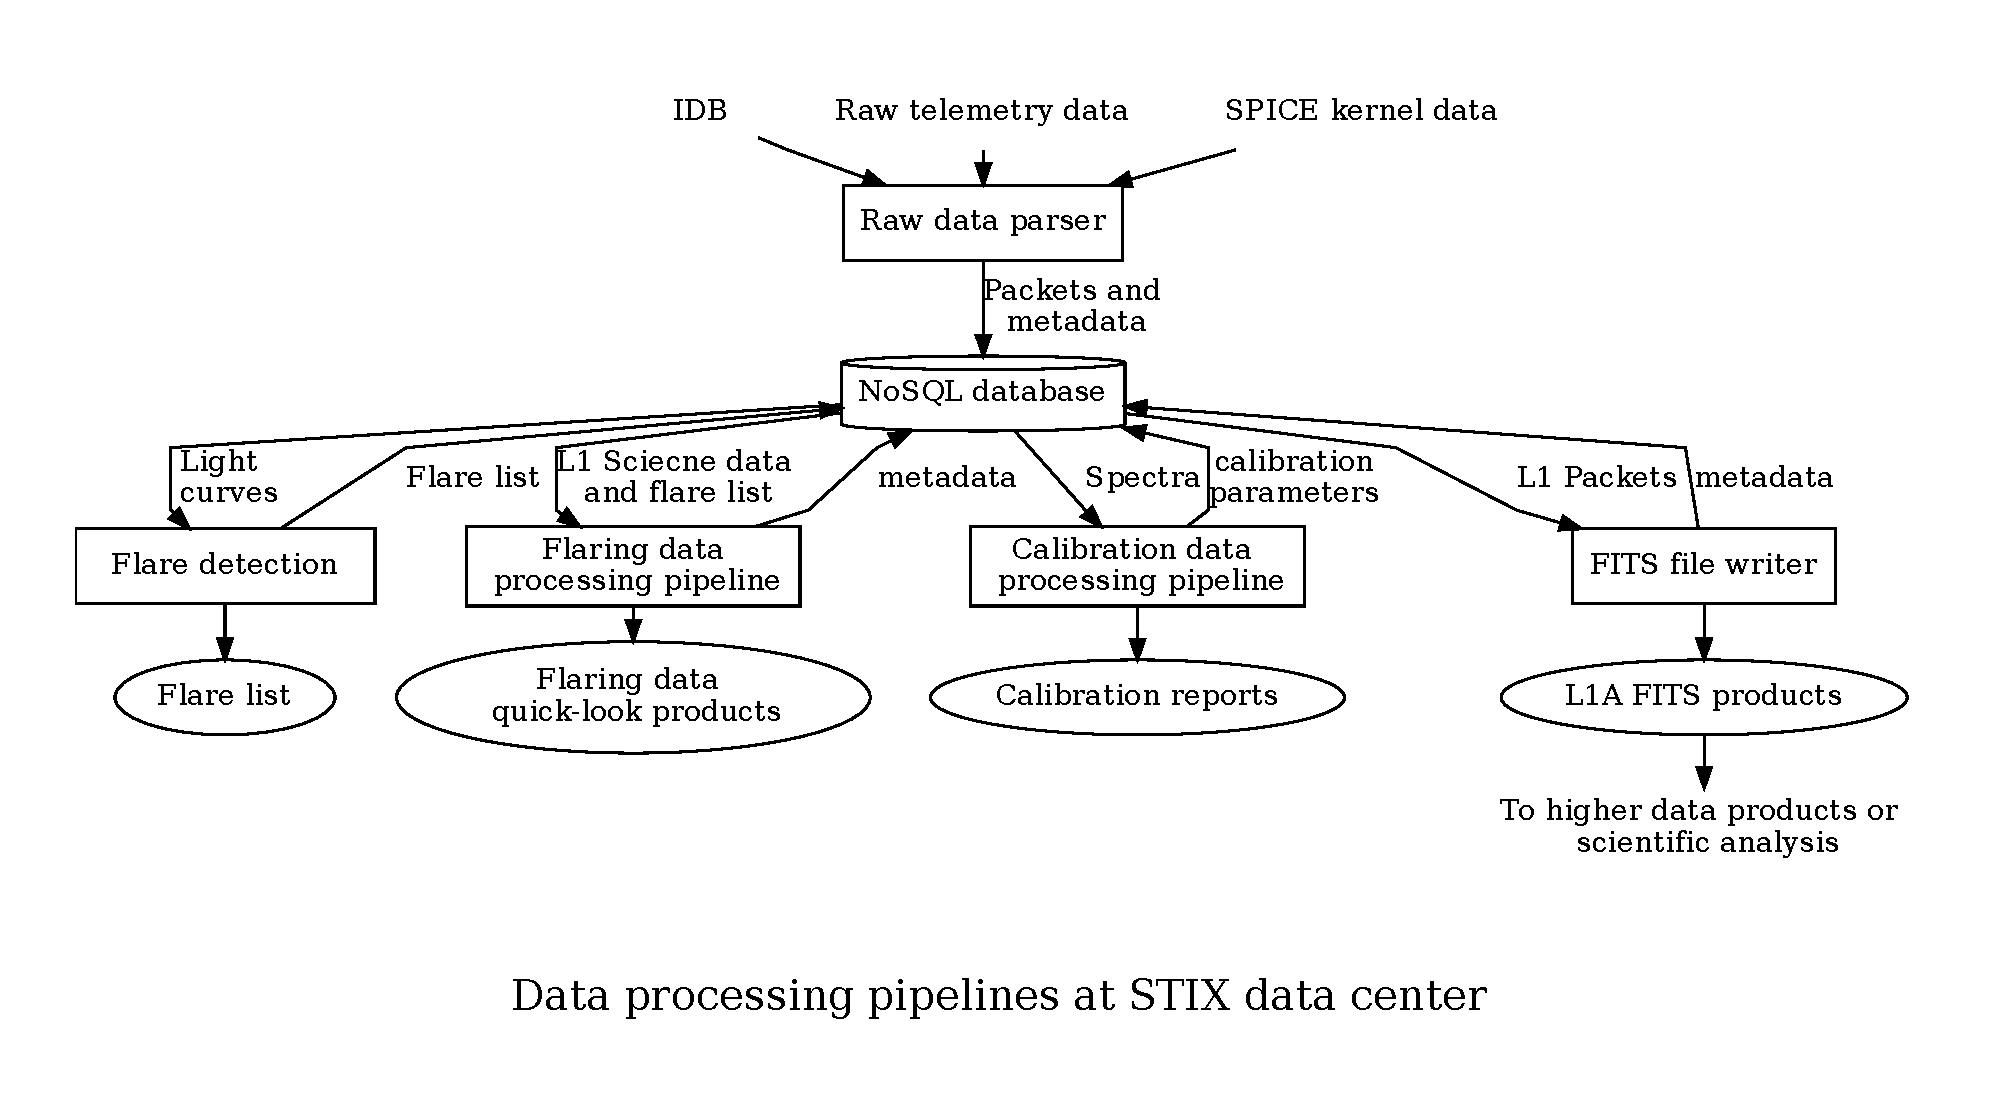
\includegraphics[width=0.9\textwidth]{figures/pipelines.pdf}
    \caption{Telemetry processing pipelines at STIX data center.}
    \label{fig:main_pipelines}
\end{figure*}
New telemetry data arrive at the STIX data center and are processed immediately by the data processing pipeline  
as shown in Fig. \ref{fig:main_pipelines}. 
It starts with level-1 processing of raw packets, which includes several steps such as  packet parsing, 
integer decompressing and timestamp converting. 
Packets after the processing are at the L1 level, they are written to a NoSQL database. 
Then they are selected and processed in four different paths. 
In the first path,  housekeeping, quick-look, and science data are successively selected and 
used to create level-1 FITS files. The second path selects calibration data for the determination
 of energy calibration factors. 
 In the third path, quick-look packets are selected and used to identify solar
flares; The fourth path performs standard analysis of science data for flares.

\subsection{Raw packet parsing and database}
Telemetry data that arrived at the STIX data center are binary packets. 
Each packet contains a fixed-length header 
and a list of parameters that vary with the type of packet. 
The parsing of parameters is based on the information in 
the mission interface database (MIB), which contains the name and the 
length of each parameter for each type of packet. 
Packets after parsing contain raw values of parameters, 
which need converting to physical values. 
Raw values of spacecraft-local times are converted to UTC times by using 
the latest version of SPICE kernels (\cite{spice1996,spice2018});
Raw values of housekeeping parameters are converted to physical values using 
the pre-calibrated conversion factors in the MIB. For compressed counts, 
they are decompressed using a look-up table. 

The raw and physical values of parameters of each packet as well as its header are grouped  
in a tree-like structure.  They are considered level-1 packets and written to a NoSQL database. 
NoSQL database is schemaless,  making it ideal for storing data with complex
structures but small sizes, like STIX level-1 packets.  
The use of the NoSQL database provides great convenience for checking the integrity of the data packet,
finding a specific data packet, merging of packets, and for the subsequent analysis of STIX data.  
In addition to level-1 packets, 
other metadata such as the raw filenames,  the version of SPICE kernel data, the version of the MIB,
a  summary of the packets are 
also written to the NoSQL database during the parsing of packets. 

\subsubsection{Creation of level-1 FITS files}
Flexible Image Transport System (FITS) is a portable file standard widely used in the astronomy 
community to store, transmit and manipulate scientific images, tables, and associated data (\cite{fits}).  
Therefore, the FITS format is adopted by the STIX data center to store standard data products. 
After the parsing of each new raw telemetry file, housekeeping, quick look, and science packets  
are sequentially selected from the NoSQL database and merged after passing checks for data integrity and consistency. 
The merged data as well as the associated metadata and auxiliary data are written to FITS files, and 
the metadata is also written to a collection in NoSQL in the meantime, which allows for fast queries on the files.
At the STIX data center, files created from the level-1 packets are considered level-1A data products. 

Level-1A FITS files are created automatically by the pipeline, and available at the STIX data center within minutes 
after the reception of the data. They are used in some of the subsequent data processing pipelines.
As predicted ephemeris data might be used when creating the Level-1A files,
FITS files are recreated after a few days to weeks after all resources are validated.
The created files are official Level-1  at the STIX data center. 
\subsection{Energy calibration}
%STIX performs energy calibration onboard by using an energy look-up table, 
%which has to be
\begin{figure}
 \centering
  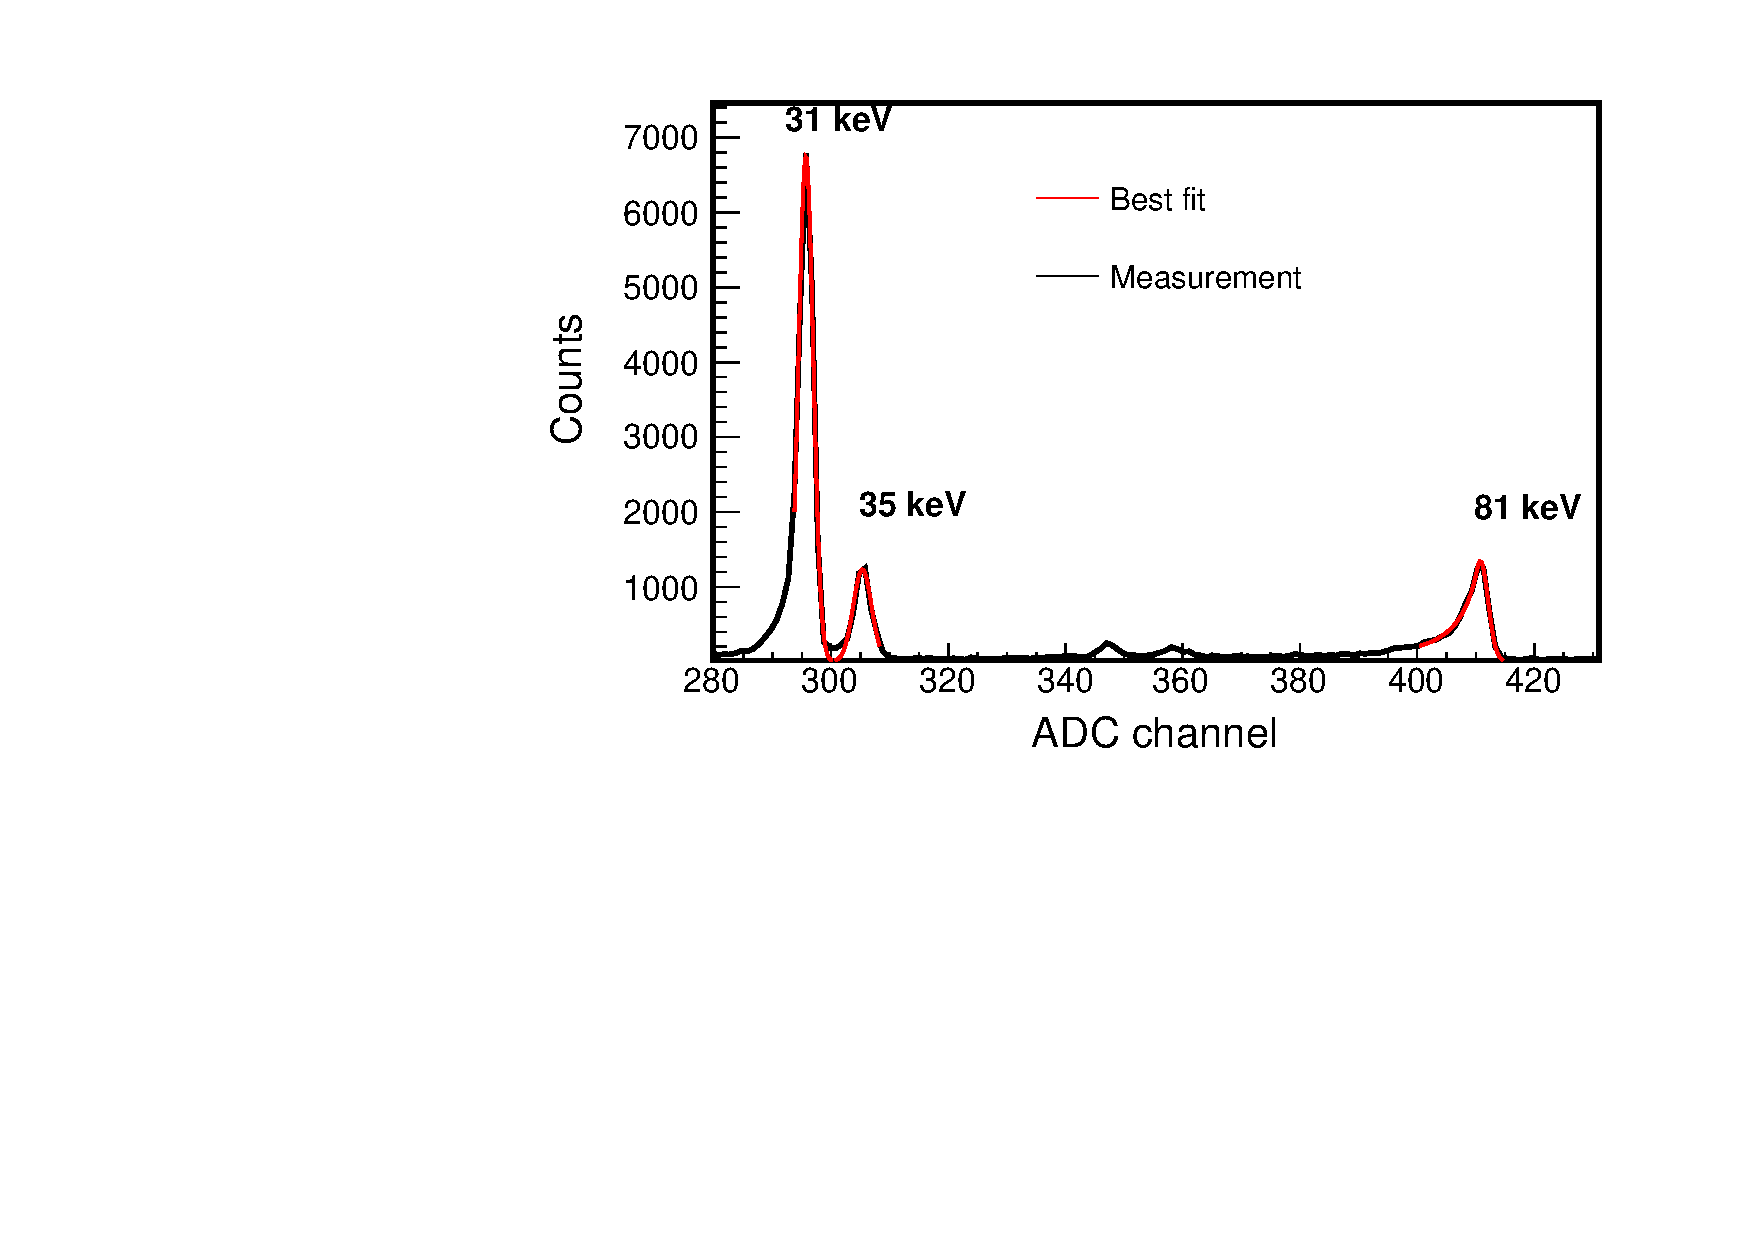
\includegraphics[width=0.8\linewidth]{figures/cal-fit.pdf}
  \caption{An example of STIX in-flight calibration count spectrum.
  The most prominent peaks, from left to right, are photopeaks of 31 keV, 35 keV, and 81 keV
  photons. The first two peaks are fitted by the double-Gaussian function and the high energy peak by  
  the crystal-ball function. }
    \label{fig:cal-fit}
\end{figure}
STIX rebins detected energies to 32 broader science energy channels onboard
with an energy look-up table (ELUT), which can be constructed using energy conversion
factors determined from calibration runs. 
STIX acquires a high-resolution calibration spectrum
for the Ba$^{133}$ sources onboard for each pixel about every 24 hours. 
The right panel of Fig.~\ref{fig:cal-fit} shows an example of the calibration spectrum of a pixel accumulated for 24 hours.  
The three most prominent peaks are produced by the photons of  31 keV, 35 keV, and 81 keV emitted by the calibration sources. 
To determine the positions of the photopeaks, we fit the first two peaks with the double-Gaussian function and the third peak
with the crystal-ball function (\cite{crsystallball}),  which consists of a Gaussian core portion 
and a power-law low-end tail, below a certain threshold.
Then we perform a linear fit of the positions and the photon energies, 
which gives the gain, namely, the ADC to energy conversion factor and the baseline. 
Another calibration spectrum fitting method often used by the STIX team  
 is the ECC method (see \cite{ecc,ecc2})).  We find that the results of the two methods are consistent at 1$\sigma$.

The above steps are performed for each calibration spectrum automatically once the data is available at the STIX data center. 
 The results are written to a dataset in the NoSQL database. 
 They are used to further correction of energy bins for science data.  
Once significant changes in the calibration factors are 
observed,  a new energy lookup table is created 
and then uploaded to STIX.


\subsection{Solar flare identification}

STIX identifies solar flares onboard based on the
 count rates of the BKG detector and other detectors.
The rough time ranges and locations of identified flares are included in the QL data.
However,  they only provide limited information on flares due to the constraints of telemetry 
bandwidth and onboard computing resources. Moreover, microflares are not identified on-board 
due to the relatively high trigger threshold.

\begin{figure}
  \centering
  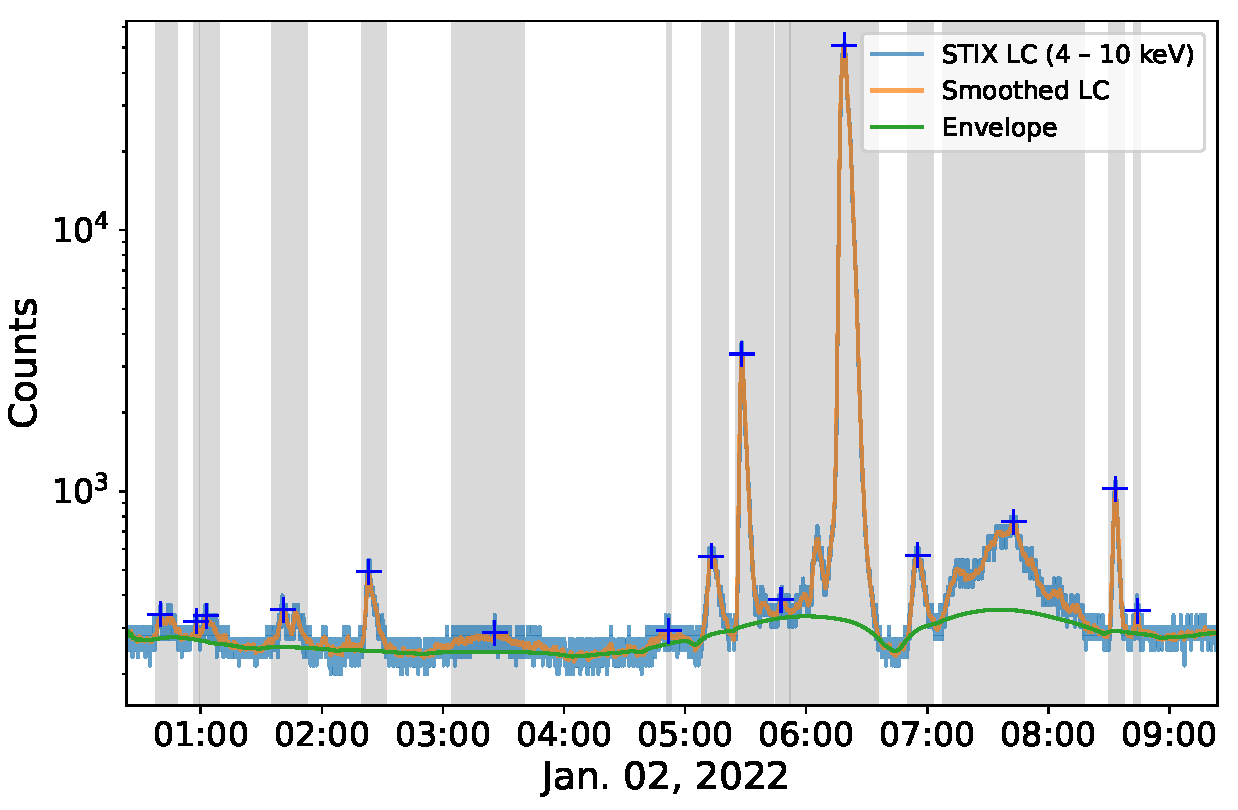
\includegraphics[width=0.8\linewidth]{figures/flaredet.pdf}
  \caption{STIX 4 -- 10 keV QL light curve recorded from 2022-08-10T21:00:00Z to 2022-08-10T18:00:00Z and 
  identified flares.   The orange curve is the smoothed light curve using a moving average filter with a time window
  of 1 minute.  The identified peaks are marked with plus signs, and the colored ranges show their time ranges.
  }
  \label{fig:flare-det}
\end{figure}
Using QL light curves, solar flares can be identified in greater detail on the ground. 
The ground flare identification procedure includes the following steps:
\begin{itemize}
  \item Light curve smoothing. The selected light curve is filtered using an unweighted
  moving average filter with a time window of 1 min. This can smooth out statistical fluctuations and electric surge spikes;
  \item Envelope subtraction.  
   A flare may last hours, and there may be short-duration pulses lying on the main pulse in the light curve.
   The main pulse is the 'envelope' of those short-duration pulses.
  To identify those short-duration pulses and estimate their durations, 
  The envelope is estimated using the Statistic-sensitive Non-linear Iterative Peak-clipping algorithm \cite{sinp}, which is widely used in X-ray spectroscopy.
    Then it is subtracted from the smoothed light curve.
  \item Identification of flare peaks. We consider a flare is detected 
 if the peak count rate after envelope subtraction lies beyond two standard deviations 
 of the mean count rate during quiet Sun periods. 
  The flare start and stop times are given at the times crossing the threshold.  
  \item Merging of flare peaks. Two flares are considered as one flare if their peak times are less than 5 minutes,
\end{itemize}

As an example, Fig.~\ref{fig:flare-det}  shows  STIX QL  light curve  in the energy range 4 -- 10 keV, recorded from 
2022-08-10T10:00:00Z to 2022-08-10T18:00:00Z.  The orange curve is the smoothed light curve using a moving average filter with a time window
of 1 minute. 
The identified peaks are marked with plus signs, and colored ranges show their time ranges.


The above steps are repeated for QL light curves of the other four higher energies
in the same time frame, which provides information on the upper limit of the X-ray energy produced by the flare.
Time ranges, peak count rate, and total counts as well as the corresponding ephemeris data of identified flares are 
written to the flare list dataset in the NoSQL database.

%\subsection{Estimation of background level}
%As mentioned earlier, a threshold value calculated using background data needs to be provided when

\subsection{Solar flare standard analysis pipeline}
\subsubsection{Estimation of solar flare GOES class }
\begin{figure}
  \centering
  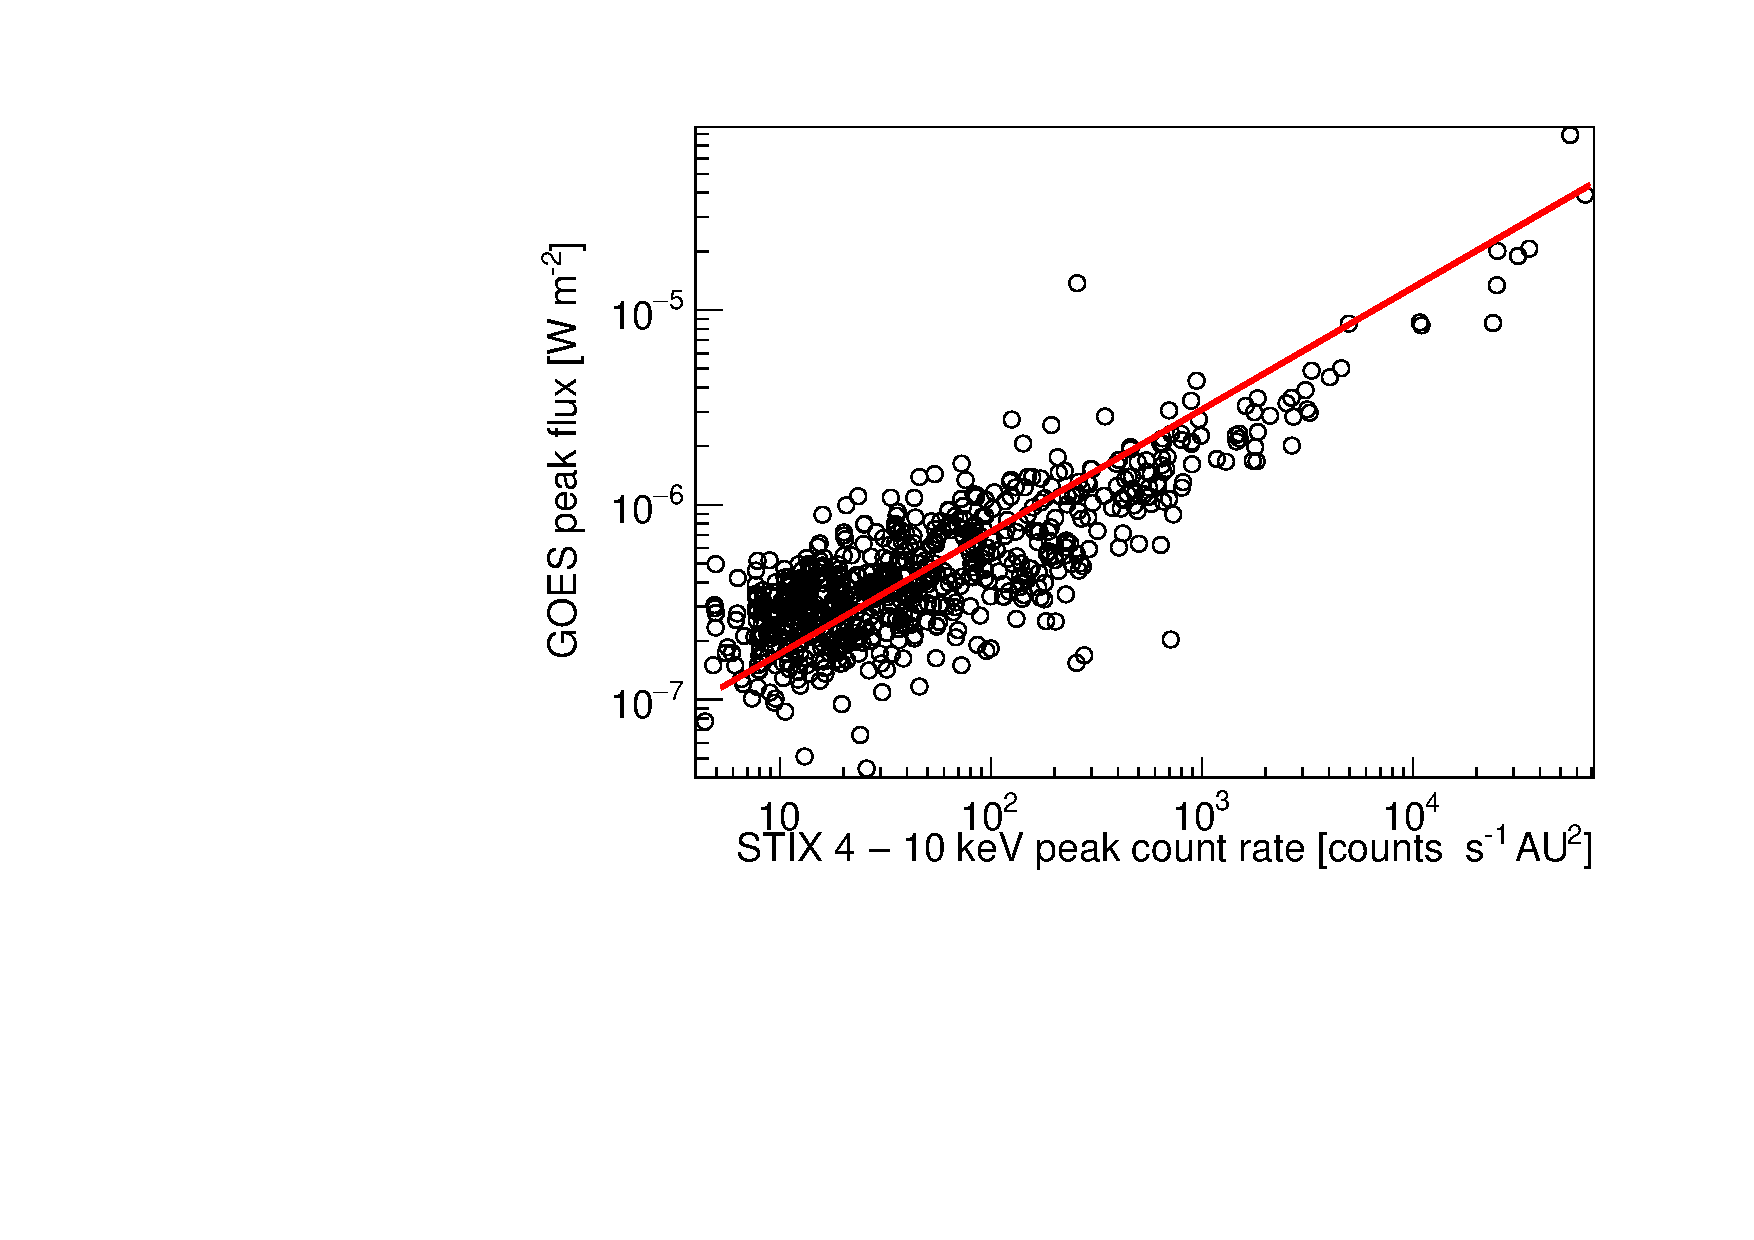
\includegraphics[width=0.8\linewidth]{figures/goes_stix_flux_paper.pdf}
  \caption{Scatter plot of GOES low channel peak flux with respect to the equivalent  peak count rate  at 1 AU
   in the 4 -- 10 keV range
  for 717 solar flares observed by both GOES and STIX duration of the commissioning phase. 
  The solid line is a linear fit to the log-log graph. 
From the fit, we obtained 
the GOES flux (in units of W/m$^2$) $f = 10^{0.622 -7.376 \log_{10} (X^{'})}$,
where $X^{'}$ is the STIX peak count rate corrected for the distance variations between the Sun and Solar Orbiter. 
}
\label{fig:goes-stix}
\end{figure}
the Sun from different angles. Therefore, a considerable number of flares observed by STIX
 are not observed by GOES satellites(and vice versa). 
In order to estimate the GOES classes of those flares, 
we selected 717 solar flares observed by both GOES and STIX in 2021. 
Fig.~\ref{fig:goes-stix} shows the scatter plot of the peak flux
measured by GOES satellites
 with respect to the STIX background-subtracted peak count rate in the energy range of 4 to 10 keV. 
It should be noted that the STIX count rate 
has been corrected for 
the different distance between Solar Orbiter and the Sun using $X^{'}=x r^2$, where $X$ is the count rate after background subtraction
 and $r$ is the distance between the Solar Orbiter and the Sun in units of AU. 
As can be seen in the figure, there is a clear correlation between
them.  The widespread at low fluxes can be explained by the difference in 
the energy response of the two instruments and the variation in flare temperatures. 
From a linear fit to the correlation in the log-log scale, 
we obtained the GOES flux in units of W/m$^2$ $\log_{10}(f) = 0.622 -7.376 \log_{10} (X^{'})$.
The above formula is currently used to estimate GOES classes of the flares
which are not directly observed by GOES satellites.  
Estimated GOES flare classes are stored in the flare list in the database. 


\subsubsection{Estimation of coarse flare locations using CFL data}
The CFL subcollimator consists of a front grid with
a distinctive pattern that selectively illuminates pixels of a 
dedicated detector based on the source location, which allows
estimating the location of the flare centroid using only the counts of the 12 pixels 
of that detector. 
Flare location is estimated onboard by maximizing the correlation between observed CFL pixel counts with expected counts using a look-up table. 
With the science data downloaded from STIX,
the coarse flare location can be reconstructed on the ground. 
This allows for more sophisticated algorithms, greater flexibility in selecting time and energy range to be integrated, and more careful background subtraction.

After receiving the pixel data for a flare, 
the coarse flare location is estimated automatically, which includes a few steps: 1) integrate counts around the peak for each CFL pixel; 
2) subtract the background 
using a background file, and 3) calculate the illuminated area of each CFL pixel based on the 
counts recorded by the CFL detector and the imaging detectors. The pixel-summed illuminated area of the imaging detectors is independent of the source location. 4) The coarse flare location is estimated by minimizing the weighted sum of squared deviations (i.e. weighted chi-squares) between the calculated illuminated areas and expectations simulated for potential flare locations in a 400 $\times$ 400 grid.
\begin{figure*}
  \centering
  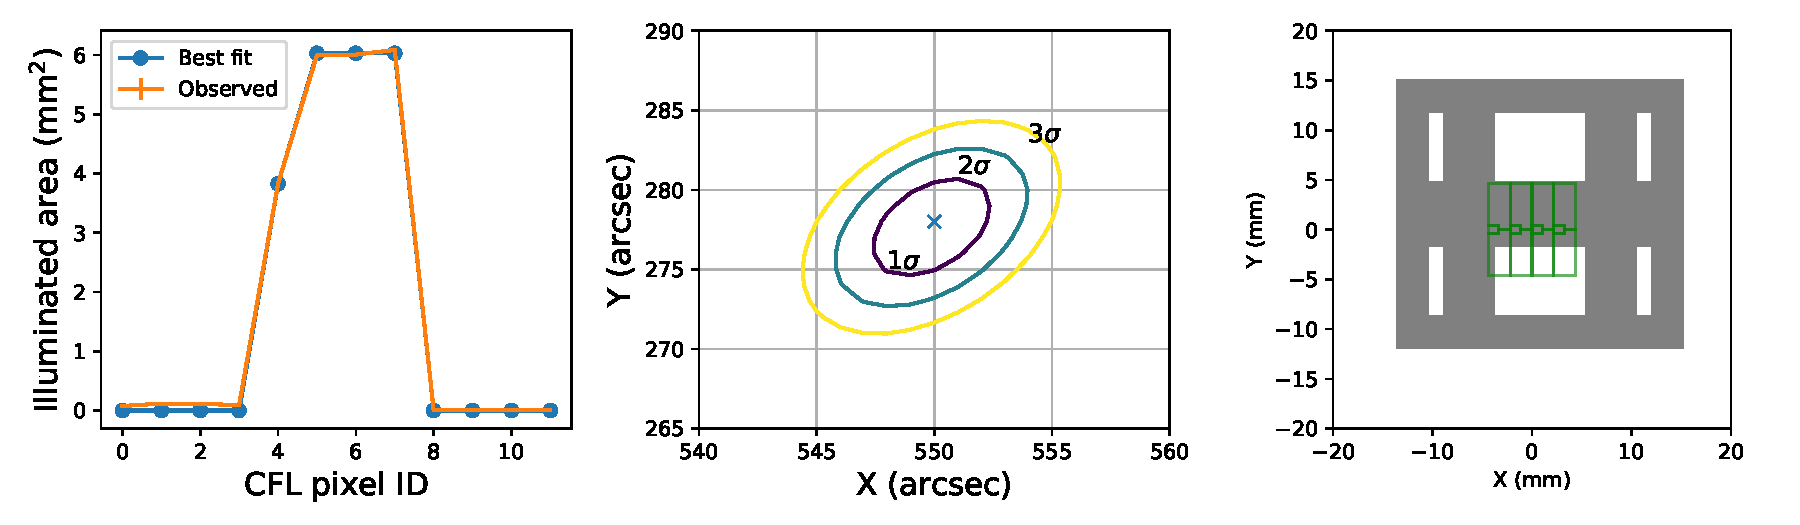
\includegraphics[width=0.95\linewidth]{figures/cflMay07.pdf}
  \caption{
   Left: Calculated areas of illuminated regions of 12 CFL pixels and the best fit simulated pattern for the flare location at (550, 278) arcsec. Pixels 0 to 3 are the top big pixels, Pixels 4 to 7 are the bottom pixels, and 8 to 11 are the small pixels as shown in the right panel.
   Middle: Best-fit flare centroid location (marked by x) and its 1$\sigma$, 2$\sigma$, and 3$\sigma$ confidence contours.
    Right: Projection of  CFL sub-collimator (the gray shaded regions) on the detector 
  simulated for the best-fit flare location. }
  \label{fig:cfl}
\end{figure*}
As an example, the left panel of Fig.~\ref{fig:cfl} shows the calculated and best-fit illuminated areas of the CFL pixels observed for STIX flare 2105071900 (GOES class M3.9);  the middle panel shows the best-fit 
flare centroid location, as well as its $1\sigma$, $2\sigma$, and $3\sigma$ contours. 
The simulated shadow of the CFL sub-collimator is shown in the right panel. 
Flare location sources are stored in the flare list in the database. 

\subsubsection{Imaging and spectroscopy pipeline}
\begin{figure*}
  \centering
  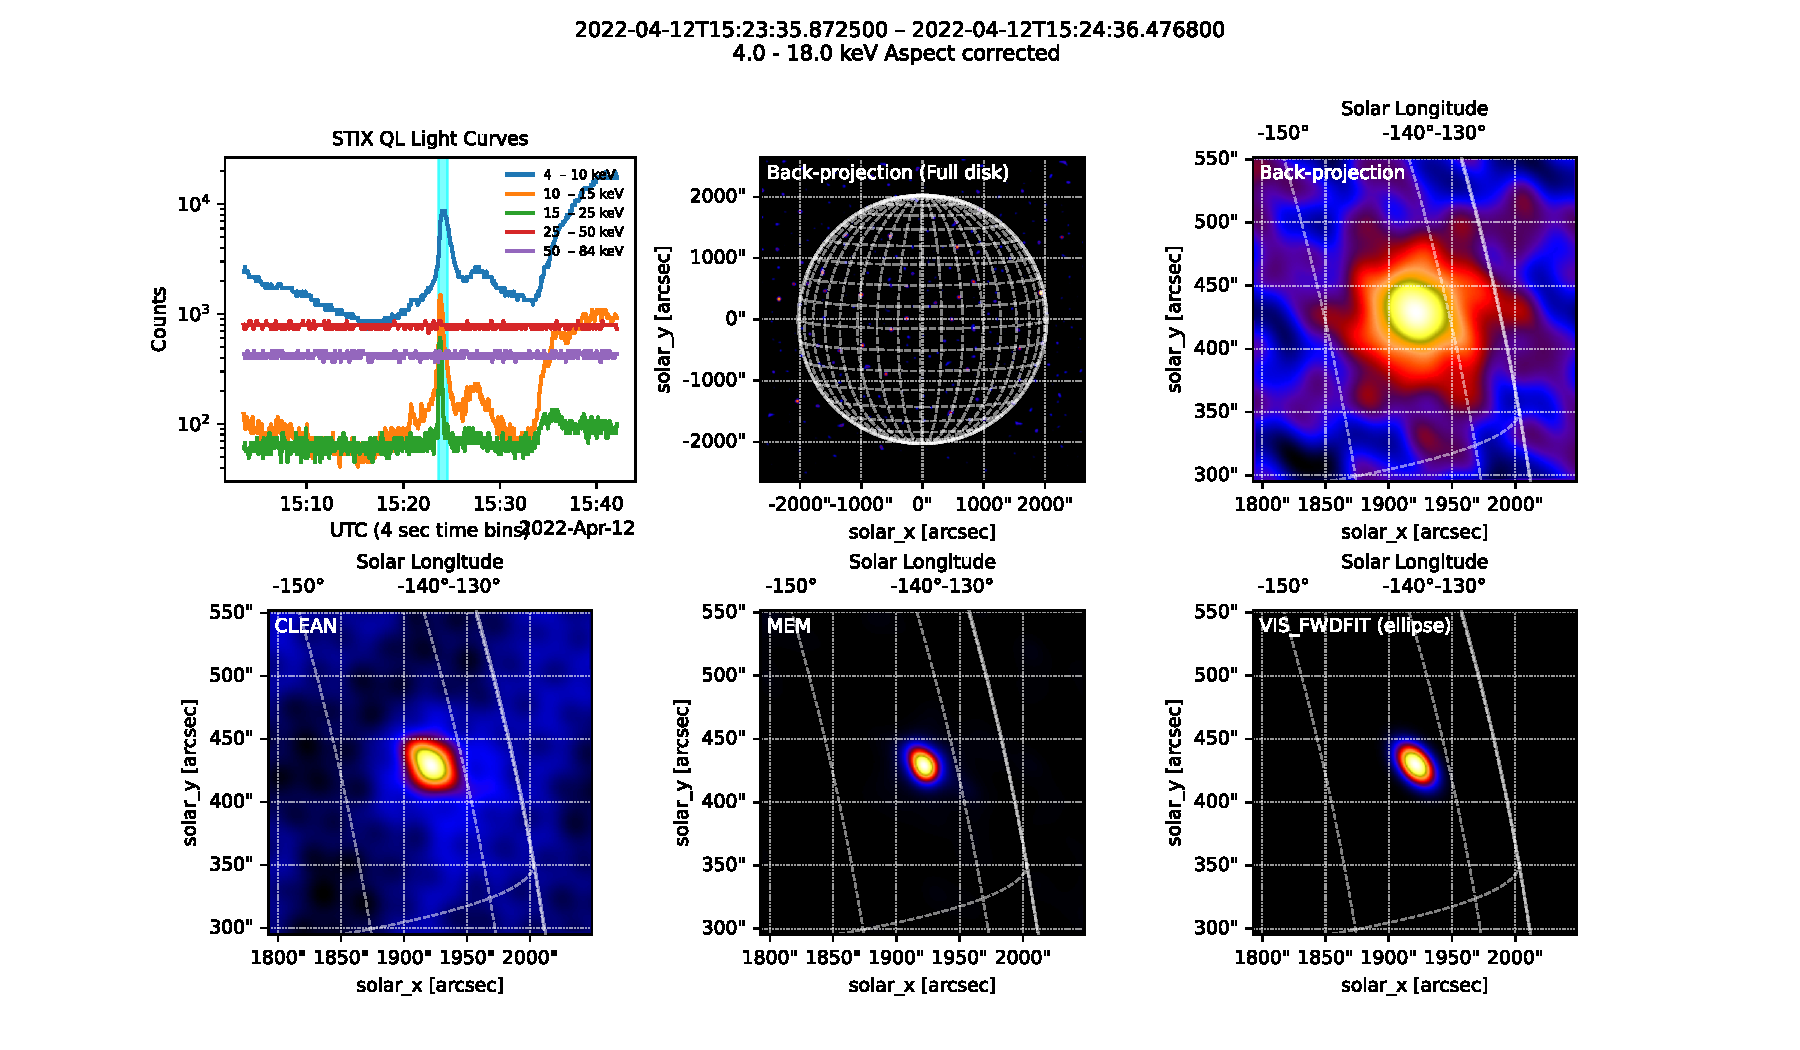
\includegraphics[width=0.95\linewidth]{figures/imaging_pipeline.pdf}
  \caption{ 
   STIX Quick-look light curves and reconstructed images of the solar flare observed at 2022-03-08T08:55:17Z, 
   created by the image reconstruction pipeline.  The period at the peak was selected and 
   Back-projection, CLEAN, EM, and VIS\_FWFIT
    algorithms were used for reconstructing images. Image products are accessible
   at the STIX data center.}
  \label{fig:imaging}
\end{figure*}
STIX detects thousands of solar flares each year. However, only
 a part of them is analyzed in detail by solar physicists. 
To facilitate the finding of flares of interest, a flare imaging and spectroscopy pipeline has been developed and integrated into the main data processing pipeline at the STIX data center.  
For each flare in the flare list, pixel counts around the flare peak (60 sec integration time) are selected. The background is then subtracted from the integrated counts using pixel data acquired in a quiet Sun period.  
After background subtraction, visibilities are calculated for two energy bands, 4 -- 10 keV (thermal) and 16 -- 28 keV (non-thermal) with the counts, which have been corrected for the transmission of materials in front of detectors and the dead time of the readout electronics. It is worth mentioning that details on the transmission and dead-time correction methods will be published in future papers. 
The images are subsequently reconstructed from the visibilities 
with the four different algorithms: Back-projection, CLEAN, 
MEM and VIS\_FWDFIT \cite{paolo2020,clean, mem}.
Reconstructed images are further corrected for STIX off-pointing and spacecraft rotations by using the auxiliary data. As an example,  the first panel of Fig. ~\ref{fig: imaging} shows the light curves and time range selected for a flare that occurred at about 2022-03-08T08:55:17Z.
The rest of the panels show the images reconstructed with different algorithms. 
After image reconstruction, the background subtracted energy spectrum for the same time range  is fitted with a thermal component, or also with a nonthermal component ~\ref{andrea2021} if the statistics in the non-thermal energy range are high enough.  Fig.~\ref{fig:ospex} shows an example of the spectral analysis results.
Imaging and spectral analysis are carried out for each identified flare automatically.  
The results are written in both FITS and PNG formats, and their 
file indexing information, parameter values from spectral analysis, and auxiliary data are stored in the NoSQL database.

\begin{figure}[h]
  \centering
  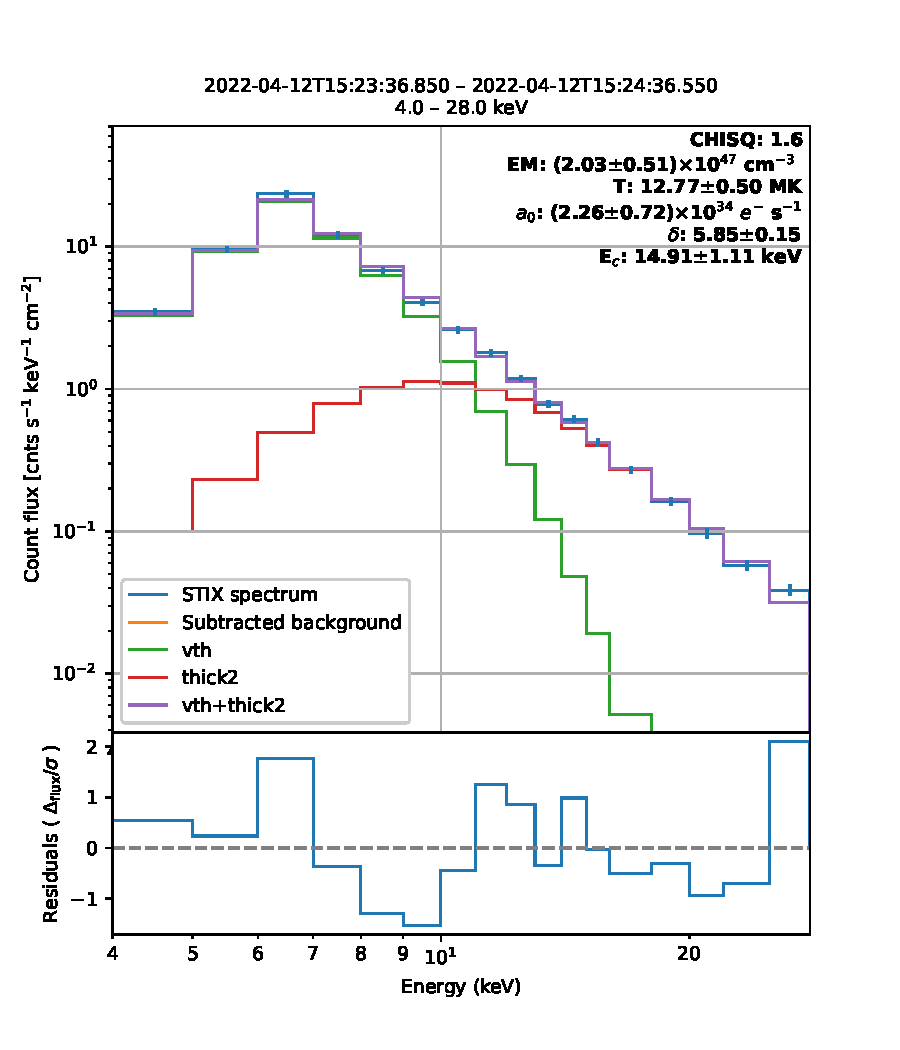
\includegraphics[width=0.9\linewidth]{figures/ospex.pdf}
  \caption{An example of spectral fitting results. 
    The imaging and spectroscopy pipeline performs
    spectral analysis for all flares in the flare list. }
  \label{fig:ospex}
\end{figure}
\section{Science data request strategy}
As mentioned earlier, the STIX data center receives low-latency data within days, whereas 
the high-resolution pixel data are stored in the onboard archive memory for about four to six months, 
before they are overwritten by new data. They are processed and down-linked 
after receiving data request telecommands from the ground. 
A data request telecommand contains information about the selected data and values of parameters
required to process the data onboard, including the data compression level, 
time range, minimal time bin, energy bin width, 
and  masks indicating detectors and pixels to be selected. 
%Their values are chosen on the basis of the knowledge of QL light curves. 
STIX data detect thousands of flares per year; therefore, 
selecting data and choosing parameter values
are tedious tasks. They must take into account many factors, 
such as count rates, time binning of data, statistics of selected data, 
and also the telemetry budget, based on the knowledge obtained from QL light curves. 
After more than two years of operation,  we have automatized the selection of data
and the strategy is as follows:
\begin{itemize}
  \item  
 Compression level-1 pixel data are requested for each of the ground-identified  flares with a total number of signal counts in the QL light curves greater than 10000, which is approximately the minimum counts to reconstruct an X-ray image. 
The requested energy range is chosen to be the range in which obvious signal counts are seen,  
whereas the requested time resolution is adjusted based on the amount of data allocated. 
If the peak count rate is above 125 counts/sec (approximately 
equivalent to the count rate observed for a B3 flare at 1 au),  pixel counts with high time resolution are requested.  Otherwise, pixel counts are integrated over the whole flaring time 
to reduce the telemetry data volume. 
 \item  Spectrograms with the highest time and energy solution (compression level 4) are requested for all periods when STIX is in observation mode. 
 \item Time-integrated pixel data for background subtraction:
Time-integrated pixel data with durations of one or two detector temperature cycles (each cycle lasts about 40 minutes), which are acquired during quiet-Sun periods, are requested. 
The data are used for background subtraction when performing spectroscopy and imaging. 
\item High time-resolution aspect data are requested for periods when the aircraft's attitude changes drastically.
Such periods can be known from the SPICE kernels or the aspect system readouts in housekeeping data. 
\end{itemize}
Requests of the types described above are created automatically on a regular basis.
Moreover, the STIX operations team also creates data requests for special needs. 
Parameter values and some descriptive information about data requests are stored in a dedicated collection in the NoSQL database.  A unique ID with a naming convention of {\it yymmddxxxx} is assigned to each newly created request, where 
the first eight digits indicate the data start time, 
and the last four digits as a whole is a random number.  
%The unique IDs are used to track the status of  requests. 
After being checked and adjusted by the STIX operations team, data requests 
 are selected from the database and then compiled into instrument operation requests (IORs). 
They are used to create the final telecommands at the mission operations center (MOC). 
An IOR is typically executed after two to three weeks of submission to ESA. 

\section{STIX data platform user interfaces}
\subsection{Interactive web pages}
\begin{figure}[h]
  \centering
  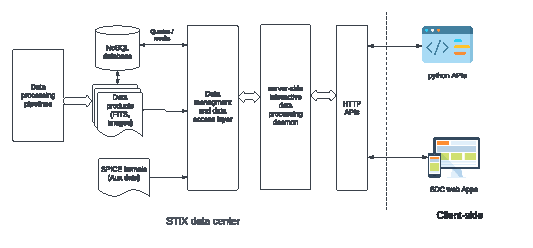
\includegraphics[width=0.9\linewidth]{figures/interfaces.pdf}
  \caption{ 
    Data flow at STIX data center.
  }
  \label{fig:interfaces}
\end{figure}

\begin{figure*}[h]
  \centering
  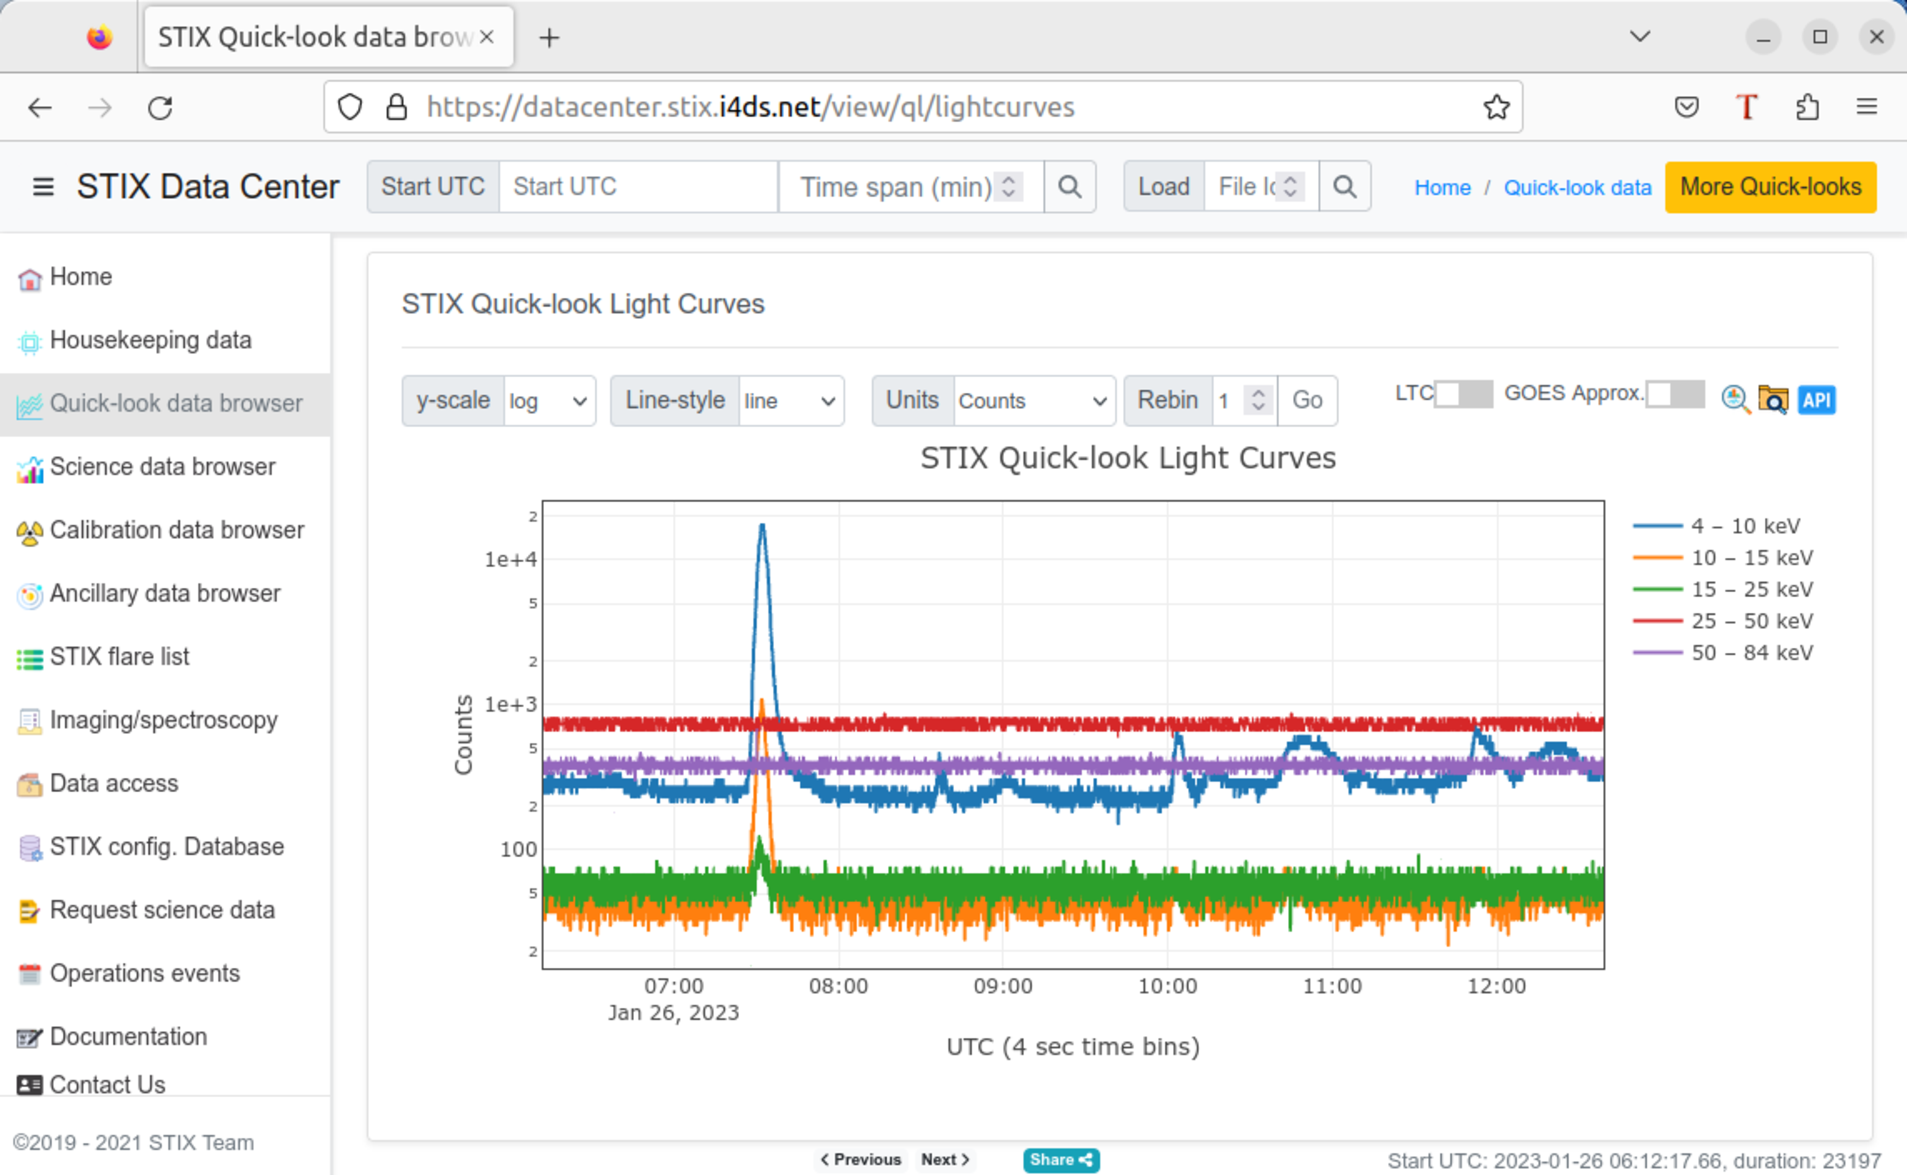
\includegraphics[width=0.7\linewidth]{figures/data-browser.pdf}
  \caption{ 
    Interactive web-based STIX Quick-look data browser. 
    In addition to STIX Quick-looks, it can also display quick-looks of simultaneous measurements 
    performed by other instruments, such as GOES X-ray fluxes, SDO/AIA images, and Solar Orbiter EUI. 
    The browser is available at the link \url{https://datacenter.stix.i4ds.net/view/ql/lightcurves}.}
  \label{fig:qlbrowser}
\end{figure*}
The data center provides a variety of APIs that allow users and applications to access STIX data products
and the data collections in the database.
The APIs accept HTTP requests from clients and send the results back after processing on the server side. 
Based on the APIs, we have built dozens of web applications to manage and browser STIX data. 
Web techniques are chosen because they offer a number of advantages, such as clear cross-platform 
usability, wide access through browsers, rapid development, and easy maintenance.

As an example, Fig.~\ref{fig:qlbrowser} shows a screenshot of the STIX Quick-look data browsing 
tool. It allows users to browse available Quick-look data interactively. It 
interacts with the server through APIs. 
After receiving a request from the client side, the server retrieves QL counts of five different energy bands from the NoSQL database for the time range specified by the user. After excluding duplicates and merging, the server sends QL counts and metadata in JSON format back to the client. The client-side browser uses the information to create interactive light curve plots using Javascript. 
The interactive plot uses state-of-the-art web technologies to enable users to perform a range of operations, such as rebinning the integration time, correcting the light travel time between the spacecraft and the Earth, and exporting data to local files. In addition to STIX quick-looks, the same page can also display quick-looks from other solar-observing instruments, making it easier to find events of interest for joint analysis.

Based on similar concepts, tens of web tools have been developed for 
browsing other STIX data products. The four most commonly used tools are listed below: 
\begin{itemize}
  \item  Science data manager and browser: It provides users with tools not only for visualizing science data, but also for searching, downloading, and analyzing science data. The interactive analysis tools allow users to interactively select data of interest for common analysis tasks such as background subtraction and energy rebinning without installing additional software. The algorithms are implemented client-side using JavaScript. 
 Additionally, users can use these tools to submit imaging and spectroscopy tasks to the server and view the results on the same page. This reduces the barriers to exploring STIX data for new users and provides convenience for experienced users.

  \item  The preview images and spectroscopy product viewer is a web-based tool that manages reconstructed flare images and spectral analysis results. It also provides users with tools to view reconstructed solar flare images and fitting results from automated imaging and spectroscopy runs, and plot the time evolution of emission measures and temperatures, as well as create animations of x-ray images for the selected runs. In addition, users can also generate IDL or Python templates using the browser, which can be used to reproduce the results on the local machines.
  \item The auxiliary data viewer is a tool that allows the user to view auxiliary data, such as the locations of the spacecraft, its velocity, and its attitude. The viewer uses data derived from the SPICE kernel or from aspect system readouts stored on the server side.  The viewer also provides tools to calculate the looking angle of flares and the coordinates of solar limbs in STIX FOVs.
  \item  With the housekeeping browser, users can view time-series plots of all STIX housekeeping parameters, including the temperature, voltage, operation mode, memory status, etc. It provides great convenience for the instrument operations team to monitor instrument status  and for STIX data users to know instrument status at any given time.
\item 
The STIX data access page offers users a range of tools for searching and downloading STIX FITS products at different levels. 
It also provides links to tools for previewing the products. As soon as they are generated at the STIX data center, STIX data products are immediately available for access on the page.
\end{itemize}




\subsection{STIX data center interface:  stixdcpy}
{\it stixdcpy} is a python package that facilitates access to and analysis of STIX data. 
With stixdcpy, users can easily query and download the data products available at the STIX data center.
Similarly to the web tools, stixdcpy also provides python modules to perform some common analysis of STIX data, such as dead time correction, transmission correction, data clipping and merging. 
stixdcpy is still under active development. As a result, its features and 
capabilities may change over time. It is always a good idea to check the project's documentation 
or website for the latest information on its status and capabilities.
The source code of stixdcpy is hosted on the GitHub repo at \url{https://github.com/i4Ds/stixdcpy}.
\section{Summary}
\label{sec:summary}
STIX is one of ten instruments onboard the Solar Orbiter,
which was launched into space on February 10, 2020.
 STIX measures the spectrum and takes X-ray images of solar 
 flares in the energy range of 4 -- 150 keV.  
 During nominal operations, STIX continuously generates telemetry data. 
 To process and archive data as well as to support the operation of 
 instruments and scientific activities using STIX data, 
 automated data processing pipelines and data platforms have been 
 developed for STIX. The pipelines generate telemetry at different levels and perform common scientific analyses.  The platform provides 
 all STIX data products of different levels and also provides users 
 with various web-based tools to search for,  browser STIX data products. 
 It also provides web-based tools to perform common analysis tasks with STIX data. 
  The data center is designed to work in a 
 fully automatic mode with minimal human intervention. The concept has proven successful 
 and has been running continuously for more than two years.
The platform not only facilitates the operations of the instrument but also provides great support to STIX data users.



\bibliographystyle{aa}
\bibliography{citations}

\end{document}
%data records, documentsMongoDB is a type of NoSQL database that uses a document-oriented data model. 
%This means that data is stored in the form of documents, which are similar to JSON objects. These documents are organized into collections, %which are similar to tables in a relational database. A MongoDB database can contain one or more collections, and each collection can contain %any number of documents.
